\section{Verifica e validazione}
La verifica e la validazione sono due attività fondamentali per garantire la qualità del prodotto software.
Queste attività sono svolte durante tutto il ciclo di vita del software, e sono svolte in parallelo con le attività di sviluppo.
\subsection*{Analisi statica}
Per analisi statica si intende l'analisi del codice sorgente senza eseguirlo, per determinare se il codice sorgente rispetta 
le regole di codifica, le convenzioni adottate e per calcolare alcune metriche di qualità del codice.\\
Per l'analisi statica del codice sorgente Java ho utilizzato IntelliJ IDEA, che
durante la scrittura del codice segnala in tempo reale eventuali errori di sintassi, errori di logica, e segnala anche
se il codice scritto non rispetta alcune convenzioni di codifica imposte dal \textit{team} di sviluppo.\\

Per l'analisi statica del codice sorgente del progetto \textit{client} ho utilizzato WebStorm che, come IntelliJ IDEA,
segnala in tempo reale eventuali errori di sintassi, errori di logica.
In aggiunta, ho utilizzato \textbf{ESLint}, che è un \textit{tool} di analisi statica del codice sorgente JavaScript e
TypeScript, che permette, a prescindere dall'editor utilizzato, di segnalare eventuali errori di sintassi e di controllare
che il codice scritto rispetti le convenzioni di codifica imposte; \\

Un'altro strumento utilizzato, in modo asincrono, per l'analisi statica del codice sorgente è \textbf{SonarQube}, 
un \textit{tool} di analisi statica del codice sorgente, che permette di calcolare alcune metriche di qualità del codice,
e di segnalare eventuali problemi di codifica, e di logica.\\
SonarQube è stato integrato con Jenkins, in modo tale che ad ogni \textit{commit} sul \textit{repository}
del codice sorgente, viene eseguita l'analisi statica del codice sorgente, e vengono segnalati eventuali problemi, mantenendo 
lo storico delle analisi effettuate, evidenziano eventuali miglioramenti o peggioramenti del codice sorgente, come mostrato in 
figura \ref{fig:sonar1} e \ref{fig:sonar2}.\\

\begin{figure}[h]
  \centering
  \begin{minipage}{0.49\textwidth}
      \centering
      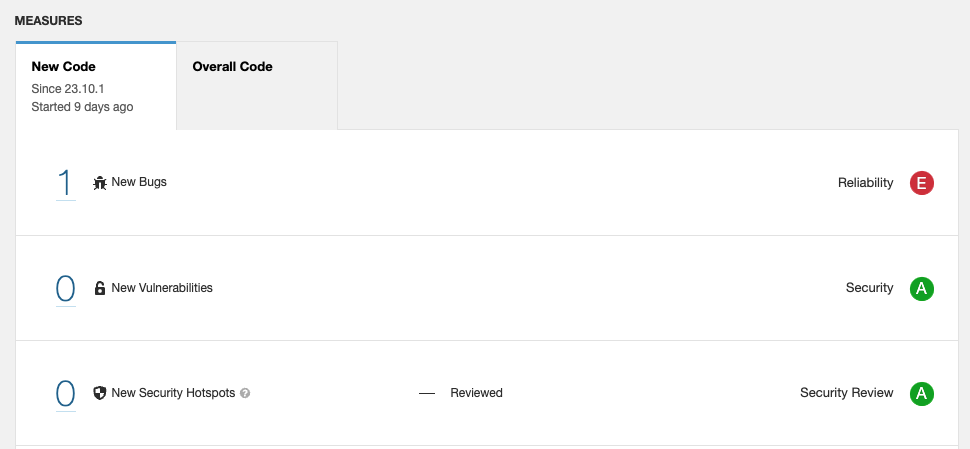
\includegraphics[width=\textwidth]{sonar1} 
      \caption{Dashboard di SonarQube.}
      \label{fig:sonar1}
  \end{minipage}\hfill
  \begin{minipage}{0.49\textwidth}
    \centering
    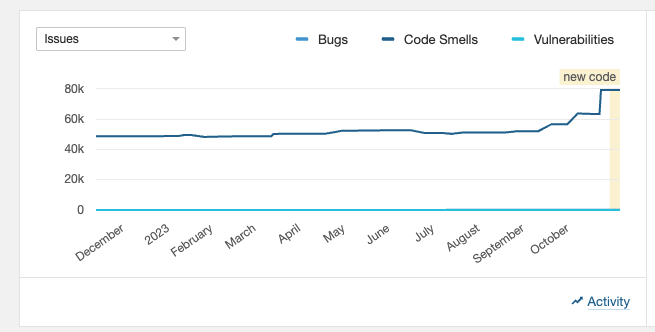
\includegraphics[width=\textwidth]{sonar2}
    \caption{Statistiche di SonarQube.}
    \label{fig:sonar2}
  \end{minipage}
\end{figure}

\subsection*{Analisi dinamica}
L'analisi dinamica è l'analisi del codice sorgente eseguendolo, per determinare se il codice sorgente rispetta
le specifiche e le aspettative.\\
Ho effettuato tre tipi di \textit{test}, i \textit{test} di unità, i \textit{test} di integrazione e i \textit{test} \textit{end-to-end}.\\
\subsubsection*{Test di unità}
I \textit{test} di unità rappresentano una componente fondamentale nello sviluppo del software, 
essenziali per garantire la qualità e l'affidabilità del codice. 
Ho adottato JUnit, un framework popolare per la scrittura di \textit{test} di unità in ambienti Java, 
per validare la correttezza delle singole unità di codice del progetto.

JUnit è stato scelto per la sua ampia adozione nella comunità Java e per la sua integrazione con gli ambienti di sviluppo e i sistemi di build che abbiamo utilizzato. La sua semplicità nell'annotare i metodi di \textit{test} e la possibilità di eseguire \textit{test} in modo ripetibile e automatizzato hanno reso JUnit lo strumento ideale per il nostro progetto.

I \textit{test} di unità sono stati implementati seguendo il principio del \textit{First Testing}: 
prima della scrittura del codice funzionale, sono stati definiti i \textit{test} per validare il comportamento atteso delle varie unità. 
Questo approccio ha contribuito a mantenere un alto standard di qualità del codice e a identificare precocemente eventuali errori.

Per ogni classe principale del progetto, è stata creata una classe di \textit{test} corrispondente. 
I \textit{test} sono stati focalizzati sulle funzionalità critiche, come la gestione delle eccezioni, 
la validazione dei dati in input e l'accuratezza dei risultati restituiti.

I \textit{test} di unità sono stati integrati nel sistema di build automatizzato, utilizzando Gradle. 
Questo ha permesso di eseguire i \textit{test} automaticamente ad ogni build, 
garantendo che eventuali regressioni o nuovi errori venissero identificati tempestivamente.

L'adozione di JUnit e l'implementazione sistematica di \textit{test} di unità hanno avuto un impatto significativo sulla qualità del software prodotto. 
I \textit{test} hanno aiutato a mantenere il codice robusto e flessibile, facilitando anche le fasi di \textit{refactoring} e l'aggiunta di nuove funzionalità. 
Inoltre, l'approccio di test-driven development ha migliorato la mia capacità di scrivere codice più chiaro e mantenibile.

\subsubsection{\textit{Test-driven development}}
Il \textit{\gls{tdd}} è una metodologia di sviluppo software che inverte l'ordine tradizionale dello sviluppo. 
Invece di scrivere prima il codice e poi i \textit{test} per verificare che il codice funzioni come previsto, nel TDD si scrivono prima 
i \textit{test} e poi il codice che deve superarli. Ecco i passaggi chiave del TDD:
\begin{enumerate}
  \item \textbf{Scrivere un test}: Prima di scrivere il codice funzionale, si scrive un \textit{test} per una nuova funzionalità. Questo \textit{test} fallirà inizialmente, poiché la funzionalità non è stata ancora implementata.
  \item \textbf{Scrivere il codice minimo necessario}: Si scrive poi il codice necessario affinché il \textit{test} passi. Questo codice non deve essere perfetto; l'obiettivo è semplicemente far passare il \textit{test} 
  \item \textit{\textbf{Refactoring}}: Una volta che il \textit{test} è superato, si procede con il \textit{refactoring} del codice. Questo passaggio consiste nel migliorare e pulire il codice senza modificarne la funzionalità, assicurandosi che i \textit{test} continuino a passare.
  \item \textbf{Ripetizione}: Questo ciclo viene ripetuto per ogni nuova funzionalità o miglioramento. Si scrive un test, si fa in modo che passi, e poi si rifinisce il codice.
\end{enumerate}

I benefici del TDD includono:
\begin{itemize}
  \item \textbf{Migliore \textit{design} del codice}: Poiché si scrive il \textit{test} prima del codice, si è spinti a pensare più attentamente a come il codice dovrebbe funzionare e alla sua interfaccia pubblica.
  \item \textbf{Codice più affidabile}: Poiché si scrive un \textit{test} per ogni nuova funzionalità, si ha una copertura di \textit{test} più ampia, il che aiuta a identificare e correggere gli errori più rapidamente.
  \item \textbf{Facilità di \textit{refactoring}}: Avendo una suite di \textit{test} che copre il codice, si può fare \textit{refactoring} con maggiore sicurezza, sapendo che i \textit{test} rileveranno eventuali regressioni introdotte.
\end{itemize}

Tuttavia, il TDD richiede disciplina e può richiedere più tempo all'inizio, 
specialmente per chi non è abituato a questa metodologia. 
Ma nel lungo termine, può portare a un codice più pulito, più facile da mantenere e con meno \textit{bug}.

\subsubsection{Test di unità per il \textit{frontend}}
Nel \textit{frontend} Angular, per la scrittura dei \textit{test} di unità mi sono affidato a \textit{Jest}, 
un \textit{framework} di testing JavaScript.
\textbf{Jest} è stato scelto per la sua ampia adozione nella comunità JavaScript 
e per la sua integrazione con gli ambienti di sviluppo e i sistemi di build che abbiamo utilizzato. 

\subsubsection*{Test di integrazione}
I \textit{test} di integrazione sono stati implementati per verificare il corretto funzionamento 
delle interazioni tra le varie componenti del sistema.
Per farlo ho utilizzato ancora JUnit, riuscendo a configurarlo in modo tale che
i \textit{test} di integrazione vengano eseguiti solo quando necessario, 
e non ad ogni \textit{build} del progetto, come invece avviene per i \textit{test} di unità.\\

Con i \textit{test} di integrazione ho verificato che tutti i servizi esposti dal \textit{backend} funzionassero correttamente,
e che il \textit{client} riuscisse a comunicare correttamente.
Nel caso dei test, il \textit{client} è stato simulato utilizzando delle chiamate \textit{HTTP} 
direttamente da codice Java, senza utilizzare il \textit{client} Angular.\\
Questo ci ha permesso di verificare che il \textit{backend} funzionasse correttamente,
senza dover dipendere dal \textit{client} Angular.

\subsubsection*{Test \textit{End-to-End}}
I \textit{test} \textit{end-to-end} sono stati l'ultimo tassello per garantire la qualità del prodotto.
Ho utilizzato \textbf{Playwright}, una libreria \textbf{Node.js} per l'automazione dei \textit{test} \textit{end-to-end}
 per applicazioni \textit{web}, sviluppata da \textbf{Microsoft}.\\
Playwright è stato scelto per la sua ampia adozione nella comunità di \azienda{},
e perchè non prevede nessun piano di abbonamento, a differenza di tanti altri.

L'obiettivo dei \textit{test} \textit{end-to-end} è quello di simulare l'interazione di 
un utente con il sistema, e verificare che il sistema funzioni correttamente.\\
Un prerequisito per l'esecuzione dei \textit{test} \textit{end-to-end} è che il sistema sia in esecuzione
e che il \textit{server} \textit{web} sia raggiungibile.\\
Per questo motivo, i \textit{test} \textit{end-to-end} sono stati eseguiti in un ambiente di \textit{staging},
in modo tale da poter simulare l'interazione di un utente con il sistema, senza dover dipendere
dall'ambiente di produzione.\\

Durante l'esecuzione dei \textit{test} \textit{end-to-end} è possibile abilitare la modalità \textit{debug},
in modo tale da poter visualizzare l'esecuzione dei \textit{test} in tempo reale, e poter intervenire
in caso di errori o sospendere l'esecuzione per analizzare lo stato del sistema.\\

In caso di errori, Playwright permette di catturare uno \textit{screenshot} della pagina,
in modo tale da poter analizzare l'errore e capire la causa anche in un secondo momento.\\
